\documentclass[border=6pt]{standalone}
\usepackage[T1]{fontenc}
\usepackage{courier}
\usepackage[scaled=0.95]{helvet}
\renewcommand{\familydefault}{\sfdefault}
\usepackage{sfmath}
\usepackage[version=4]{mhchem}
\usepackage{tikz}
\usepackage{pgfplots}
\pgfplotsset{compat=newest}
\usetikzlibrary{arrows.meta,positioning,calc,fit,backgrounds,shapes.geometric,decorations.pathreplacing,patterns}
\definecolor{ink}{HTML}{17233A}
\definecolor{inksoft}{HTML}{44506A}
\definecolor{teal}{HTML}{0E6B6B}
\definecolor{tealsoft}{HTML}{E5F0EF}
\definecolor{amber}{HTML}{B26B12}
\definecolor{ambersoft}{HTML}{FBF0DF}
\definecolor{blue}{HTML}{2F6690}
\definecolor{bluesoft}{HTML}{E3ECF4}
\definecolor{plum}{HTML}{7A4D8C}
\definecolor{plumsoft}{HTML}{EFE7F3}
\definecolor{greyc}{HTML}{8A94A3}
\definecolor{linec}{HTML}{D3DCE1}
\definecolor{oxy}{HTML}{C0392B}
\definecolor{carb}{HTML}{3B4252}
\definecolor{hyd}{HTML}{E6E9EE}
\definecolor{nit}{HTML}{2F6690}
\tikzset{
  every picture/.style={line cap=round,line join=round},
  lab/.style={font=\small, text=inksoft},
  >={Stealth[length=7pt]},
}
\pgfplotsset{
  every axis/.append style={axis line style={inksoft}, tick style={inksoft}, tick label style={font=\footnotesize, text=inksoft}, label style={font=\small, text=ink}},
}
% fragment tile: \frag{node name}{position}{colour}{content}
\newcommand{\frag}[4]{\node[draw=#3, fill=#3!12, line width=1.4pt, rounded corners=6pt, minimum width=1.25cm, minimum height=1.05cm, text=#3, font=\bfseries] (#1) at (#2) {#4};}
\newcommand{\ring}{\tikz[baseline=-0.6ex]{\draw[line width=1.1pt] (0:0.3)--(60:0.3)--(120:0.3)--(180:0.3)--(240:0.3)--(300:0.3)--cycle; \draw[line width=0.8pt] (0,0) circle (0.16);}}
\newcommand{\bond}[2]{\draw[ink, line width=2.2pt] (#1) -- (#2);}

\begin{document}
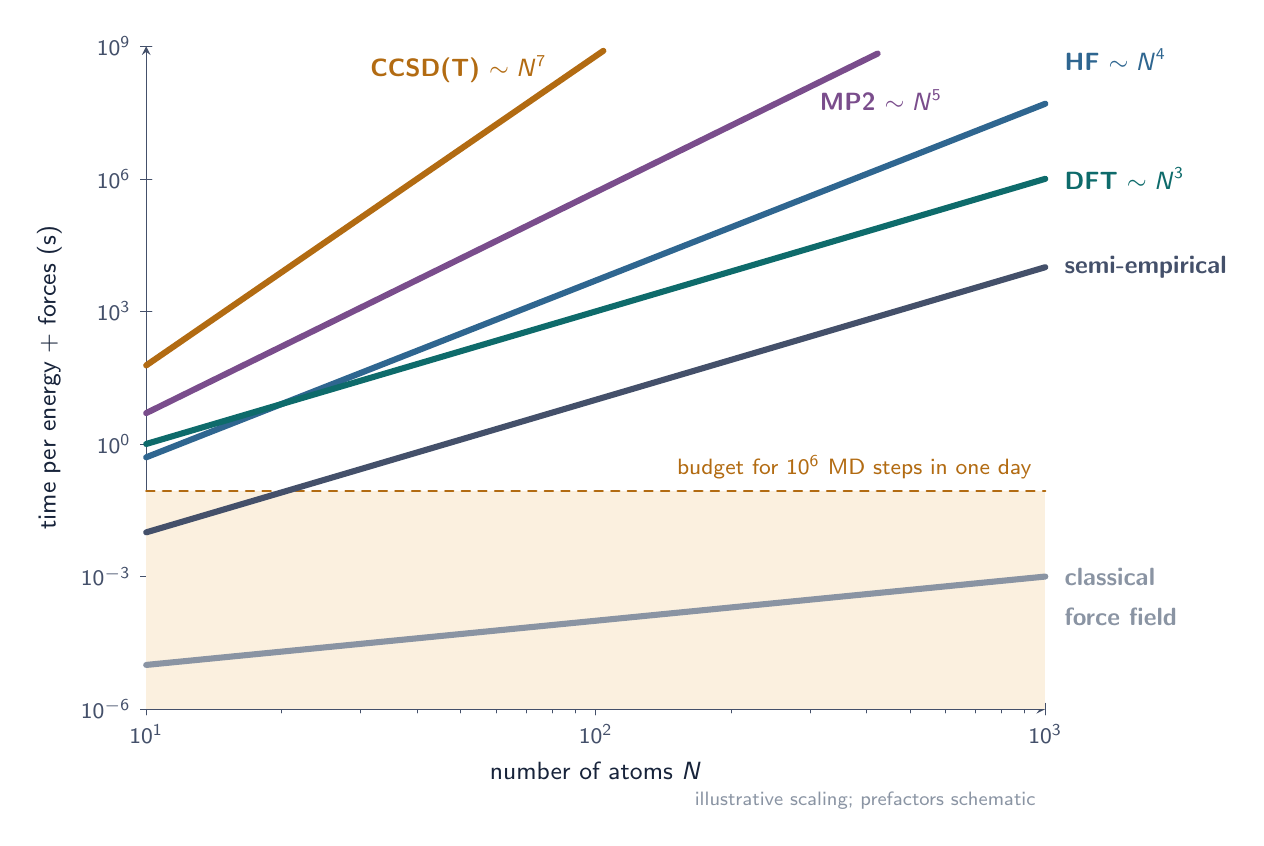
\begin{tikzpicture}
\begin{axis}[width=13cm,height=10cm,xmode=log,ymode=log,xmin=10,xmax=1000,ymin=1e-6,ymax=1e9,
  axis lines=left, xlabel={number of atoms $N$}, ylabel={time per energy + forces (s)},
  ytick={1e-6,1e-3,1,1e3,1e6,1e9}, clip=false]
\fill[ambersoft] (axis cs:10,1e-6) rectangle (axis cs:1000,0.086);
\draw[amber, dashed, thick] (axis cs:10,0.086) -- (axis cs:1000,0.086);
\node[text=amber, font=\footnotesize, anchor=south east, align=right] at (axis cs:980,0.1) {budget for $10^6$ MD steps in one day};
\addplot[amber, line width=2.2pt] coordinates {(10,60) (10.812,103.62) (11.69,178.95) (12.638,309.04) (13.664,533.71) (14.774,921.7) (15.973,1591.8) (17.27,2749) (18.672,4747.4) (20.188,8198.7) (21.826,14159) (23.598,24452) (25.514,42229) (27.585,72928) (29.825,1.2595e+05) (32.246,2.1751e+05) (34.864,3.7563e+05) (37.694,6.4871e+05) (40.754,1.1203e+06) (44.062,1.9348e+06) (47.639,3.3413e+06) (51.507,5.7703e+06) (55.688,9.9653e+06) (60.209,1.721e+07) (65.097,2.9721e+07) (70.381,5.1328e+07) (76.095,8.8643e+07) (82.272,1.5308e+08) (88.951,2.6437e+08) (96.172,4.5657e+08) (103.98,7.8849e+08)};
\addplot[plum, line width=2.2pt] coordinates {(10,5) (10.812,7.3869) (11.69,10.913) (12.638,16.123) (13.664,23.82) (14.774,35.191) (15.973,51.99) (17.27,76.809) (18.672,113.48) (20.188,167.65) (21.826,247.68) (23.598,365.91) (25.514,540.59) (27.585,798.66) (29.825,1179.9) (32.246,1743.2) (34.864,2575.3) (37.694,3804.7) (40.754,5621.1) (44.062,8304.4) (47.639,12269) (51.507,18126) (55.688,26778) (60.209,39562) (65.097,58448) (70.381,86349) (76.095,1.2757e+05) (82.272,1.8847e+05) (88.951,2.7844e+05) (96.172,4.1136e+05) (103.98,6.0774e+05) (112.42,8.9786e+05) (121.55,1.3265e+06) (131.41,1.9597e+06) (142.08,2.8952e+06) (153.62,4.2773e+06) (166.09,6.3192e+06) (179.57,9.3359e+06) (194.15,1.3793e+07) (209.91,2.0377e+07) (226.95,3.0104e+07) (245.38,4.4476e+07) (265.29,6.5707e+07) (286.83,9.7075e+07) (310.12,1.4342e+08) (335.29,2.1188e+08) (362.51,3.1303e+08) (391.94,4.6246e+08) (423.76,6.8322e+08)};
\addplot[blue, line width=2.2pt] coordinates {(10,0.5) (10.812,0.68322) (11.69,0.93359) (12.638,1.2757) (13.664,1.7432) (14.774,2.382) (15.973,3.2548) (17.27,4.4476) (18.672,6.0774) (20.188,8.3044) (21.826,11.348) (23.598,15.506) (25.514,21.188) (27.585,28.952) (29.825,39.562) (32.246,54.059) (34.864,73.869) (37.694,100.94) (40.754,137.93) (44.062,188.47) (47.639,257.53) (51.507,351.91) (55.688,480.86) (60.209,657.07) (65.097,897.86) (70.381,1226.9) (76.095,1676.5) (82.272,2290.8) (88.951,3130.3) (96.172,4277.3) (103.98,5844.8) (112.42,7986.6) (121.55,10913) (131.41,14912) (142.08,20377) (153.62,27844) (166.09,38047) (179.57,51990) (194.15,71042) (209.91,97075) (226.95,1.3265e+05) (245.38,1.8126e+05) (265.29,2.4768e+05) (286.83,3.3844e+05) (310.12,4.6246e+05) (335.29,6.3192e+05) (362.51,8.6349e+05) (391.94,1.1799e+06) (423.76,1.6123e+06) (458.16,2.2031e+06) (495.35,3.0104e+06) (535.57,4.1136e+06) (579.04,5.6211e+06) (626.05,7.6809e+06) (676.88,1.0496e+07) (731.82,1.4342e+07) (791.23,1.9597e+07) (855.47,2.6778e+07) (924.91,3.6591e+07) (1000,5e+07)};
\addplot[teal, line width=2.2pt] coordinates {(10,1) (10.812,1.2638) (11.69,1.5973) (12.638,2.0188) (13.664,2.5514) (14.774,3.2246) (15.973,4.0754) (17.27,5.1507) (18.672,6.5097) (20.188,8.2272) (21.826,10.398) (23.598,13.141) (25.514,16.609) (27.585,20.991) (29.825,26.529) (32.246,33.529) (34.864,42.376) (37.694,53.557) (40.754,67.688) (44.062,85.547) (47.639,108.12) (51.507,136.64) (55.688,172.7) (60.209,218.26) (65.097,275.85) (70.381,348.64) (76.095,440.62) (82.272,556.88) (88.951,703.81) (96.172,889.51) (103.98,1124.2) (112.42,1420.8) (121.55,1795.7) (131.41,2269.5) (142.08,2868.3) (153.62,3625.1) (166.09,4581.6) (179.57,5790.4) (194.15,7318.2) (209.91,9249.1) (226.95,11690) (245.38,14774) (265.29,18672) (286.83,23598) (310.12,29825) (335.29,37694) (362.51,47639) (391.94,60209) (423.76,76095) (458.16,96172) (495.35,1.2155e+05) (535.57,1.5362e+05) (579.04,1.9415e+05) (626.05,2.4538e+05) (676.88,3.1012e+05) (731.82,3.9194e+05) (791.23,4.9535e+05) (855.47,6.2605e+05) (924.91,7.9123e+05) (1000,1e+06)};
\addplot[inksoft, line width=2.2pt] coordinates {(10,0.01) (10.812,0.012638) (11.69,0.015973) (12.638,0.020188) (13.664,0.025514) (14.774,0.032246) (15.973,0.040754) (17.27,0.051507) (18.672,0.065097) (20.188,0.082272) (21.826,0.10398) (23.598,0.13141) (25.514,0.16609) (27.585,0.20991) (29.825,0.26529) (32.246,0.33529) (34.864,0.42376) (37.694,0.53557) (40.754,0.67688) (44.062,0.85547) (47.639,1.0812) (51.507,1.3664) (55.688,1.727) (60.209,2.1826) (65.097,2.7585) (70.381,3.4864) (76.095,4.4062) (82.272,5.5688) (88.951,7.0381) (96.172,8.8951) (103.98,11.242) (112.42,14.208) (121.55,17.957) (131.41,22.695) (142.08,28.683) (153.62,36.251) (166.09,45.816) (179.57,57.904) (194.15,73.182) (209.91,92.491) (226.95,116.9) (245.38,147.74) (265.29,186.72) (286.83,235.98) (310.12,298.25) (335.29,376.94) (362.51,476.39) (391.94,602.09) (423.76,760.95) (458.16,961.72) (495.35,1215.5) (535.57,1536.2) (579.04,1941.5) (626.05,2453.8) (676.88,3101.2) (731.82,3919.4) (791.23,4953.5) (855.47,6260.5) (924.91,7912.3) (1000,10000)};
\addplot[greyc, line width=2.2pt] coordinates {(10,1e-05) (10.812,1.0812e-05) (11.69,1.169e-05) (12.638,1.2638e-05) (13.664,1.3664e-05) (14.774,1.4774e-05) (15.973,1.5973e-05) (17.27,1.727e-05) (18.672,1.8672e-05) (20.188,2.0188e-05) (21.826,2.1826e-05) (23.598,2.3598e-05) (25.514,2.5514e-05) (27.585,2.7585e-05) (29.825,2.9825e-05) (32.246,3.2246e-05) (34.864,3.4864e-05) (37.694,3.7694e-05) (40.754,4.0754e-05) (44.062,4.4062e-05) (47.639,4.7639e-05) (51.507,5.1507e-05) (55.688,5.5688e-05) (60.209,6.0209e-05) (65.097,6.5097e-05) (70.381,7.0381e-05) (76.095,7.6095e-05) (82.272,8.2272e-05) (88.951,8.8951e-05) (96.172,9.6172e-05) (103.98,0.00010398) (112.42,0.00011242) (121.55,0.00012155) (131.41,0.00013141) (142.08,0.00014208) (153.62,0.00015362) (166.09,0.00016609) (179.57,0.00017957) (194.15,0.00019415) (209.91,0.00020991) (226.95,0.00022695) (245.38,0.00024538) (265.29,0.00026529) (286.83,0.00028683) (310.12,0.00031012) (335.29,0.00033529) (362.51,0.00036251) (391.94,0.00039194) (423.76,0.00042376) (458.16,0.00045816) (495.35,0.00049535) (535.57,0.00053557) (579.04,0.00057904) (626.05,0.00062605) (676.88,0.00067688) (731.82,0.00073182) (791.23,0.00079123) (855.47,0.00085547) (924.91,0.00092491) (1000,0.001)};

\node[text=amber, font=\small\bfseries, anchor=west] at (axis cs:30,3e8) {CCSD(T) $\sim N^7$};
\node[text=plum, font=\small\bfseries, anchor=west] at (axis cs:300,6e7) {MP2 $\sim N^5$};
\node[text=blue, font=\small\bfseries, anchor=west] at (axis cs:1050,5e8) {HF $\sim N^4$};
\node[text=teal, font=\small\bfseries, anchor=west] at (axis cs:1050,1e6) {DFT $\sim N^3$};
\node[text=inksoft, font=\small\bfseries, anchor=west] at (axis cs:1050,1e4) {semi-empirical};
\node[text=greyc, font=\small\bfseries, anchor=west] at (axis cs:1050,1e-3) {classical};
\node[text=greyc, font=\small\bfseries, anchor=west] at (axis cs:1050,1.2e-4) {force field};

\node[font=\scriptsize, text=greyc, anchor=north east] at (rel axis cs:1,-0.11) {illustrative scaling; prefactors schematic};
\end{axis}
\end{tikzpicture}
\end{document}